This systematic review was conducted by two reviewers from different institutions following the procedures as described in \cite{kitchenham:2004, Moher:2009}. 
A systematic review can be conducted for several reasons such as (a) the summarisation and comparison, in terms of advantages and disadvantages, of various approaches in a field, (b) the identification of open problems, (c) the contribution of a joint conceptualization comprising the various approaches developed in a field, or (d) the synthesis of a new idea to cover the emphasized problems. 
This systematic review comprises of all the above mentioned reasons, in that, it summarises and compares various data quality assessment methodologies as well as identifies open problems focused on Linked Open Data.
Moreover, it contributes a conceptualization of the data quality assessment field and thereafter proposes a new method for data quality assessment for LOD.

\paragraph{Related surveys.}
In order to justify the need of conducting the systematic review, we first conducted a search for related surveys and literature reviews.
We did not come across any study focused on data quality assessment methodologies and tools for Linked Data. 
However, there is a comprehensive review \cite{Batini:2006}, which surveys 13 methodologies for assessing the data quality of datasets available on the web in structured or semi-structured formats.
% what's the difference: we focus on structured data, the Linked Data field only emerged after publishing of the survey, hence, certain crucial aspects such as ... are not covered.
%LOD vs databases (information systems)
%we looked at approaches of assessing linked data 
%he focused only on dimensions
%we introduced new dimensions, metrics
%we introduced assessment steps specifically for LOD as we didn't find a standardised methodology in the approaches we came across

\paragraph{Research question.}
The goal of this review is to analyse existing methodologies for assessing the quality of structured data, with particular interest in Linked Data.
To achieve this goal, we aim to answer the following general research question: \\

\emph{What are the existing approaches for assessing the quality of Linked Data?}\\

We can divide this general research question into further fine-grained research questions such as: 
\begin{itemize}
\item		\textit{What are the problems that each approach assesses?}
\item		\textit{Which are the quality dimensions and metrics supported by the proposed approaches?}
\item		\textit{What kind of tools are available for data quality assessment?}
\item		\textit{What are the assessment methods proposed by the different approaches?}
\end{itemize}

\paragraph{Define eligibility criteria.}
The eligibility criteria is an important element of any systematic review. 
First, each member created a set of inclusion and exclusion criteria on their own. 
Second, as a result of a discussion between both members a list of eligible criteria was obtained as follows:
\begin{itemize}
\item Inclusion criteria:
\begin{itemize}
\item Studies published in English between 2002 and 2012.
\item Studies focused on data quality assessment in Linked Data	
\item Studies focused on provenance assessment of Linked Data
\item Studies that proposed and implemented an approach for data quality assessment
\item Studies that assessed the quality of Linked Data and reported issues 
\end{itemize}
\item Exclusion criteria:
\begin{itemize}
\item Studies that were not peer reviewed or published
\item Methodologies that were published as a poster
\item Studies that were focused on data quality management
\item Studies that did not focus neither on Linked Data nor on structured data
\item Studies that did non propose any methodology or framework about the assessment of quality in Linked Data
%\item Studies that did not focus on quality assessment of Linked Data but only mentions the term
\end{itemize}
\end{itemize}

\begin{figure*}[ht]
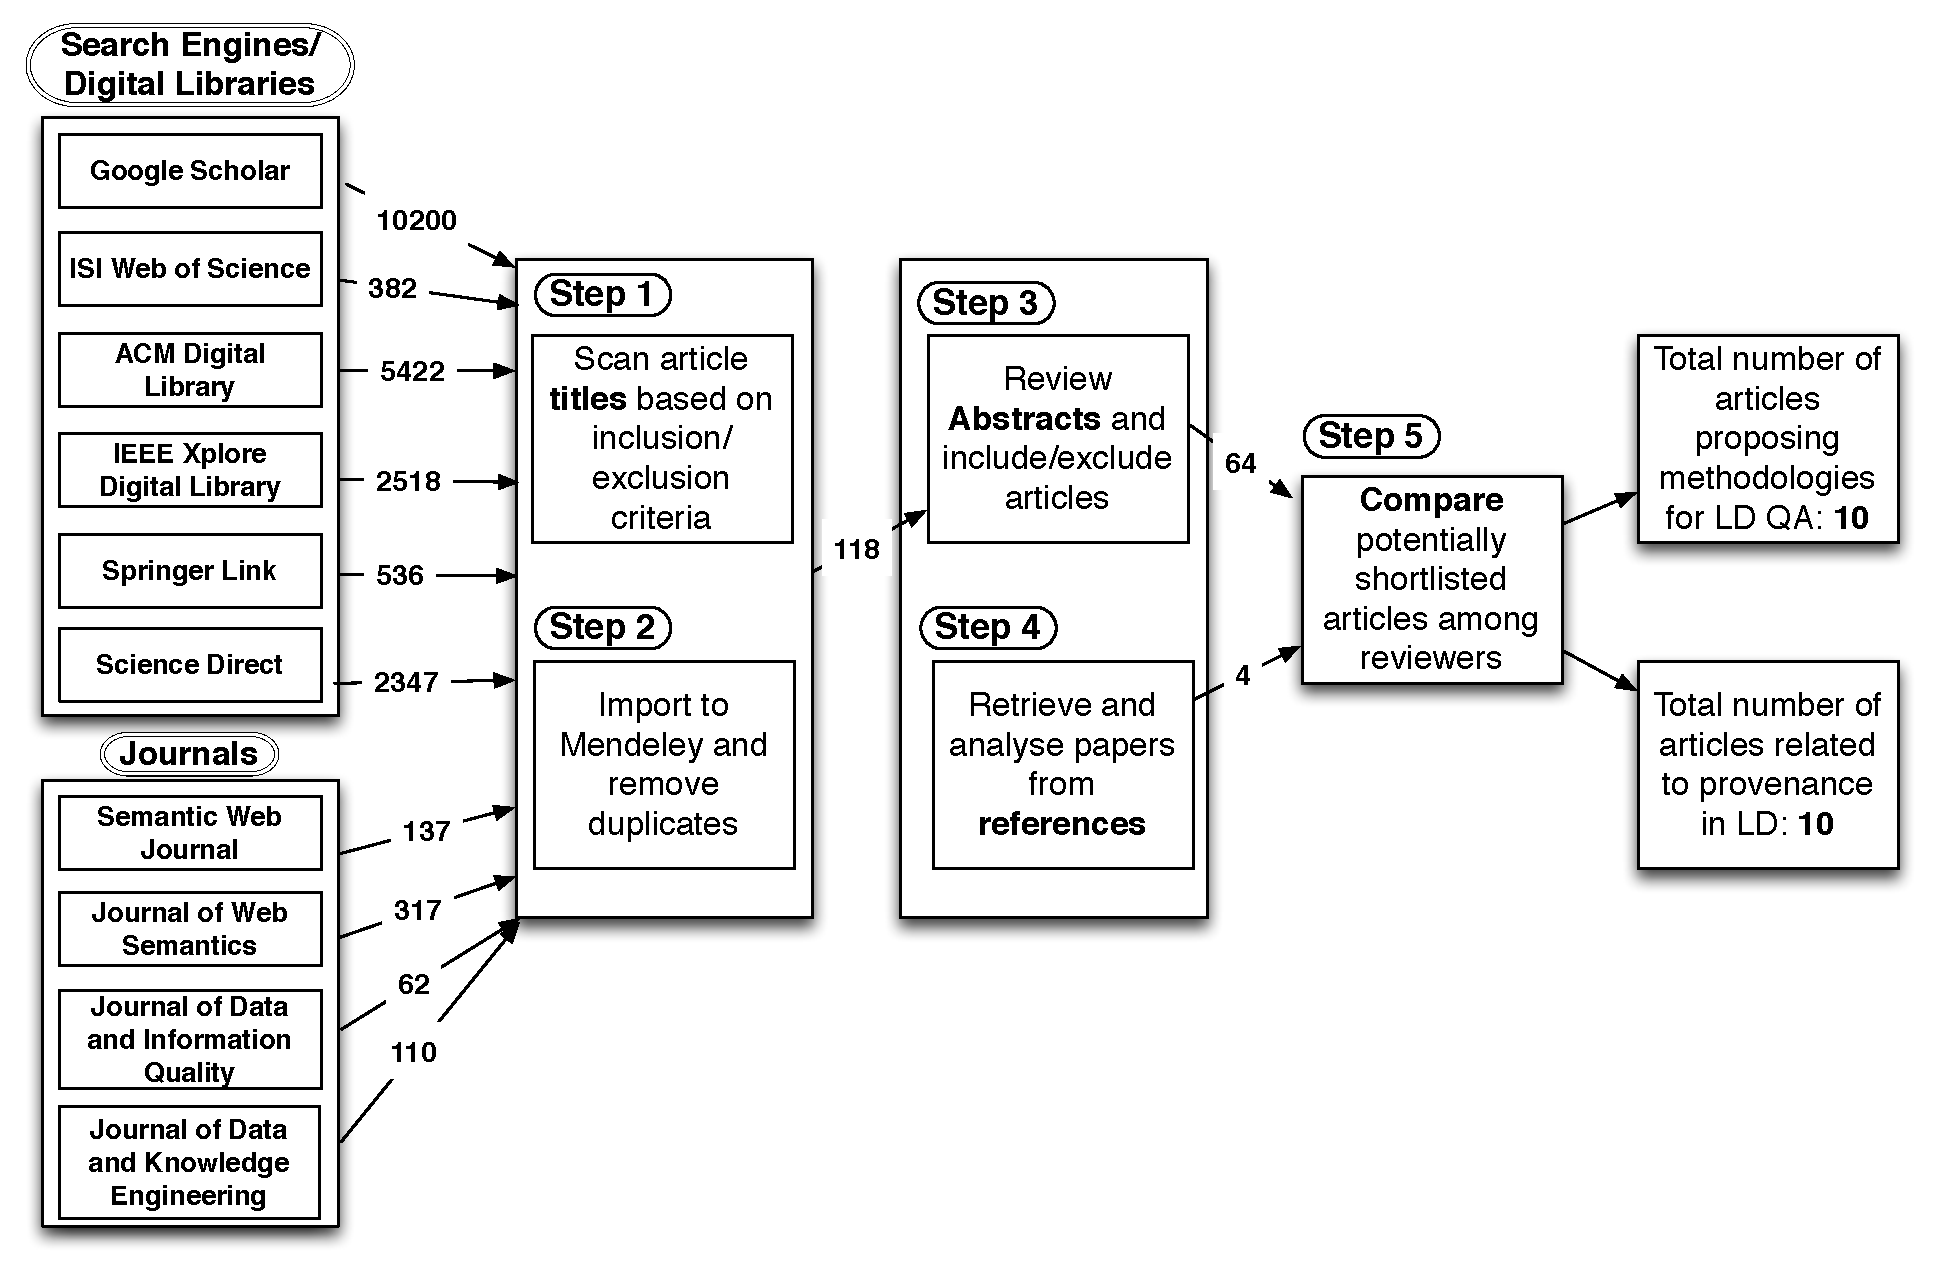
\includegraphics[width=6.5in]{Numberofarticles.pdf}
\caption{Number of articles retrieved during literature search.}
\label{fig:noofarticles}
\end{figure*}

\paragraph{Search strategy.}
Search strategies in a systematic review are usually iterative and are ran separately by both members. 
Based on the research question and the eligibility criteria, each reviewer identified several terms that were most appropriate for this systematic review, such as: \textit{data}, \textit{quality}, \textit{data quality}, \textit{assessment}, \textit{evaluation}, \textit{methodology}, \textit{improvement}, or \textit{linked data}, which were used as follows:
\begin{itemize}
\item \textit{linked data} and (\textit{quality} OR \textit{assessment} OR \textit{evaluation} OR \textit{methodology} OR \textit{improvement})
\item  \textit{data} OR \textit{quality} OR \textit{data quality} AND \textit{assessment} OR \textit{evaluation} OR \textit{methodology} OR \textit{improvement}
\end{itemize}
%The next decision was to find the suitable field (i.e. title, abstract and full-text) to apply the search
string on. 
In our experience, searching in the \textit{title} alone does not always provide us with all relevant publications. 
Thus, \textit{abstract} or \textit{full-text} of publications should also potentially be included. 
On the other hand, since the search on the full-text of studies results in many irrelevant publications, we chose to apply the search query first on the \textit{title} and \textit{abstract} of the studies.
This means a study is selected as a candidate study if its \textit{title} or \textit{abstract} contains the keywords defined in the search string.

After we defined the search strategy, we applied the keyword search in the following list of search engines, digital libraries, journals, conferences and their respective workshops: \\
Search Engines and digital libraries:
\begin{itemize}
\item Google Scholar
\item ISI Web of Science
\item ACM Digital Library
\item IEEE Xplore Digital Library
\item Springer Link
\item Science Direct
\end{itemize}
Journals:
\begin{itemize}
\item Semantic Web Journal
\item Journal of Web Semantics
\item Journal of Data and Information Quality
\item Journal of Data and Knowledge Engineering
\end{itemize}
Conferences and their Respective Workshops:
\begin{itemize}
\item International Semantic Web Conference (ISWC)
\item European Semantic Web Conference (ESWC)
\item Asian Semantic Web Conference (ASWC)
\item International World Wide Web Conference (WWW)
\item Semantic Web in Provenance Management (SWPM)
\item Consuming Linked Data (COLD)
\item Linked Data on the Web (LDOW)
\item Web Quality
\end{itemize}
Thereafter the bibliographic metadata about the 118 potentially relevant primary study were recorded using the bibliography management platform Mendeley\footnote{https://www.mendeley.com/}.

\paragraph{Titles and abstract reviewing.}
Both reviewers independently screened the titles and abstracts of the retrieved 118 articles to identify the potentially eligible articles. 
In case of disagreement while merging the lists, the problem was resolved either by mutual consensus or by creating a list of articles to go under a more detailed review. 
Then, both the reviewers compared the articles and based on mutual agreement obtained a final list of 64 articles to be included. 

\paragraph{Retrieving further potential articles.}
In order to ensure that all relevant articles were included, an additional strategy was applied such as:
\begin{itemize}
\item Looking up the reference in the selected articles
\item Looking up the article title in Google Scholar and retrieving the "Cited By" papers to check against the eligibility criteria
\item Taking each data quality dimension individually and perform a related article search
\end{itemize}
After performing these search strategies, we further retrieved 4 additional articles. 

\paragraph{Extracting data for quantitative and qualitative analysis.}
An overview of the search methodology and the number of retrieved articles at each step is shown in Figure \ref{fig:noofarticles}.
The result of the above described methodology is 21 papers from 2002 to 2012 that are reported in Table~\ref{selectedpapers} which are the core of our survey.
The next step was then to extract data from each of the articles to perform quantitative and qualitative analysis.

%\textit{To analyze the information appropriately, we required a suitable qualitative data analysis method applicable to our dataset. We used coding as our qualitative analysis methods}

\begin{table*}[htb]
\caption{List of the selected papers.} 
\label{selectedpapers}
\begin{tabular}{ | p{2.7cm} | p{10cm} | }
\hline
\textbf{Citation} & \textbf{Title} \\
\hline
Gil et.al., 2002 & Trusting Information Sources One Citizen at a Time \\
\hline
Golbeck et. al., 2003 & Trust Networks on the Semantic Web \\
\hline
Mostafavi et.al., 2004 & An ontology-based method for quality assessment of spatial data bases\\
\hline
Golbeck, 2006 & Using Trust and Provenance for Content Filtering on the Semantic Web \\
\hline
Gil et.al., 2007 & Towards content trust of web resources \\
\hline
Lei et.al., 2007 & A framework for evaluating semantic metadata \\
\hline
Hartig, 2008 & Trustworthiness of Data on the Web \\
\hline
Bizer et.al.,2009 & Quality-driven information filtering using the WIQA policy framework \\	
\hline
B\"ohm et.al., 2010 & Profiling linked open data with ProLOD \\	
\hline
Chen et.al., 2010 & Hypothesis generation and data quality assessment through association mining \\
\hline
Flemming et.al., 2010 & Assessing the quality of a Linked Data source \\
\hline
Hogan et.al., 2010 & Weaving the Pedantic Web \\
\hline
Shekarpour et.al., 2010 & Modeling and evaluation of trust with an extension in semantic web \\
\hline
F\"urber et.al., 2011 & Swiqa - a semantic web information quality assessment framework \\
\hline
Gamble et.al., 2011 & Quality, Trust, and Utility of Scientific Data on the Web: Towards a Joint Model \\
\hline
Jacobi et.al., 2011 & Rule-Based Trust Assessment on the Semantic Web \\
\hline
Bonatti et. al., 2012 & Robust and scalable linked data reasoning incorporating provenance and trust annotations \\
\hline
Gu\'eret et. al., 2012 & Assessing Linked Data Mappings Using Network Measures \\
\hline
Hogan et.al.,2012 & An empirical survey of Linked Data conformance \\
\hline
Mendes et.al.,2012 & Sieve: Linked Data Quality Assessment and Fusion \\
\hline
Rula et.al., 2012 & Capturing the Age of Linked Open Data: Towards a Dataset-independent Framework \\
\hline
\end{tabular}
\end{table*}

\paragraph{Comparison perspective of selected approaches.}
There exist several perspectives that can be used to analyze and compare the selected approaches, such as:
\begin{itemize}
\item the definitions of the core concepts
\item the dimensions and metrics proposed by each approach
\item the type of data that is considered for the assessment
\item the level of automatization of supported tools
\item the phases/steps that compose the assessment methods
\end{itemize}
Selected approaches differ in how they consider all of these perspectives and are thus compared and described in Section~\ref{concepts} and Section~\ref{sec:analysis}.

\section{Conceptualization}
\label{concepts}

There exist a number of discrepancies in the definition of many concepts in data quality due to the contextual nature of quality~\cite{Batini:2006} .
Therefore, we first describe and formally define the research context terminology (in Section~\ref{sec:general}) as well as the Linked Data quality dimensions (in Section~\ref{sec:dimensions}) in more detail.

\subsection{General terms}
\label{sec:general}
%A generalized architecture of data quality is depicted in Figure. 

\textbf{RDF Dataset.}
In this document, we understand a data source as an access point for Linked Data in the Web. 
A data source provides a dataset and it may support multiple methods of access.
The RDF triples, RDF graph and the RDF datasets have been adopted by the W3C Data Access Working Group \cite{Beckett:2004,Hayes:2004,Brickley2004}.

Given an infinite set $\mathcal{U}$ of URIs (resource identifiers), an infinite set $\mathcal{B}$ of blank nodes, and an infinite set $\mathcal{L}$ of literals, a triple $ \langle s, p, o \rangle \in (\mathcal{U} \cup \mathcal{B})\times \mathcal{U} \times (\mathcal{U} \cup \mathcal{B} \cup \mathcal{L})$ is called an RDF triple; where $s$, $p$, $o$ are the subject, the predicate and the object of the triple, respectively. An RDF graph $G$ is a set of RDF triples. A named graph is a pair  $\langle G,u \rangle$, where $G$ is called the default graph and $u\in\mathcal{U}$. An RDF dataset is a set of default and named graphs = $\lbrace G, (u_1,G_1), (u_2,G_2), ...(u_n,G_n)\rbrace$. 

\textbf{Data Quality.}
%WIQA
The concept of data quality is a domain-specific subconcept of the general concept of quality. 
A popular definition for quality is the "fitness for use"~\cite{qdefn}.
Data quality is commonly conceived as a multidimensional construct, as the "fitness for use" may depend on various factors such as accuracy, timeliness, completeness, relevancy, objectivity, believability, understandability, consistency, conciseness, availability, and verifiability~\cite{qconsumers}.

In terms of the Semantic Web, there are varying concepts of data quality.
The semantic metadata, for example, is an important concept to be considered when assessing the quality of datasets~\cite{Leigold}.
On the other hand, the notion of link quality is another important aspect in Linked Data that is introduced, where it is automatically detected whether a link is useful or not~\cite{Gueret}.
Also, it is to be noted that \textit{data} and \textit{information} are interchangeably used in the literature. 

\textbf{Data Quality Problems.}
%What is data quality problem? How the others have defined it?
The data quality problem refers to a set of issues that can affect the potentiality of the applications that use data. 
Bizer et al. \cite{Bizer} defines data quality problems as the choice of web-based information systems design which integrate information from different providers.  In \cite{Mendes} the problem of data quality is related to values being in conflict between different data sources as a consequence of the diversity of the data. 

In \cite{Flemming} the author does not provide a definition of it but implicitly explains the problems in terms of \textit{data diversity}. 
In \cite{Hogan} the authors discuss about \textit{errors} or \textit{noise} or \textit{difficulties} and in \cite{Hogan:2012} the author discuss about \textit{modelling issues} which are prone of the non exploitations of those data from the applications.
%
%%because it may be incomplete, poorly formatted, inconsistent,
%%What kind of problems we could have?
%%Errors which compromise the effectiveness of applications leveraging the resulting data. 
%%- Publishing errors; Incomplete; Incoherent; Poorly formatted; Inconsistent; Hijack; Dereferancability; Syntax errors; Link quality; Outdated; Incorrectness; Serialization problems; Inusability; System Problems; Inaccurate; Misleading; Outdated\\
%
%%Semantic Metadata
%%Data sources my have low quality such as misspelling, erroneous statements, etc; problems could be derived from the heterogeneity of data sources such as inconsistencies and duplicated entries; or be introduces by the tools employed. Changes to the data sources or to the underlying ontologies could also bring problems. 
%%data are modelled in a manner that is not
%%facilitative to generic consumption
%

\textbf{Data Quality Dimensions and Metrics.}
Data quality assessment involves the measurement of quality \textit{dimensions} or \textit{criteria} that are relevant to the consumer.
A data quality assessment \textit{metric} or \textit{measure} is a procedure for measuring an information quality dimension~\cite{Bizer}. 
These metrics are heuristics that are designed to fit a specific assessment situation~\cite{metric}.
Since the dimensions are rather abstract concepts, the assessment metrics rely on quality \textit{indicators} that allow for the assessment of the quality of a data source w.r.t the criteria~\cite{Flemming}.
An assessment score is computed from these indicators using a scoring function. 

In \cite{Bizer}, the data quality dimensions are classified into three categories according to the type of information that is used as quality indicator: (1) Content Based - information content itself; (2) Context Based - information about the context in which information was claimed; (3) Rating Based - based on the ratings about the data itself or the information provider. 

However, we identify further dimensions (defined in Section~\ref{sec:dimensions}) and also further categories to classify the dimensions, namely (1) Contextual (2) Provenance (3) Intrinsic (4) Accessibility (5) Representation and (6) Dataset Dynamicity, as depicted in Figure~\ref{fig:dimrel}.

\textbf{Data Quality Assessment Method.}
%WIQA
A data quality assessment methodology is defined as the process of evaluation if a piece of data meets in the information consumers need in a specific use case~\cite{Bizer}.
The process involves measuring the quality dimensions that are relevant to the user and comparing the assessment results with the users quality requirements.
%The steps involved in data quality assessment are: (1) formulating a research question; (2) selecting datasets and performing analyses; (3) detecting quality problems; (4) performing data quality analysis; (5) improving data quality and identifying short comings.
%%Semantic Metadata
%%There are three major steps involved in the evaluation procedure, including: setting up the evaluation context, detecting quality problems and calculating and analyzing the quality status. 

\begin{figure}
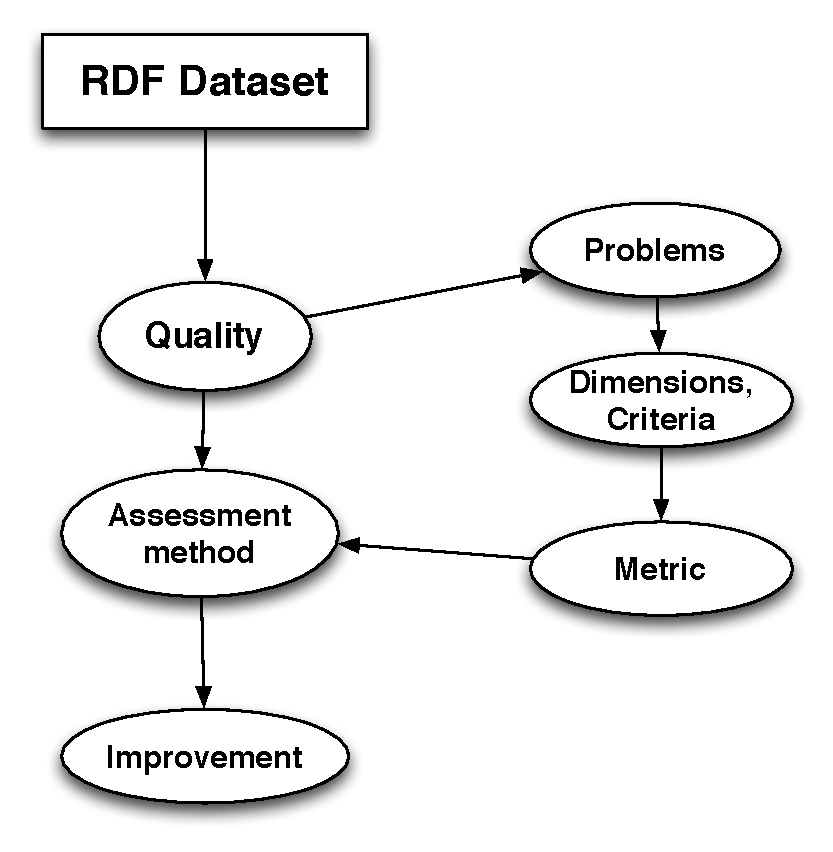
\includegraphics[scale=0.5]{Mindmap.pdf}
\caption{Conceptualization of the data quality domain.}
\label{fig:mindmap}
\end{figure}

\subsection{Linked Data quality dimensions}
\label{sec:dimensions}
% prior definitions
% our definition
%* example
%* relation to other quality dimensions
% Introduce and explain the 6 super classes of the dimensions: intrinsic, contextual, provenance, accessibility, representation, dataset dynamicity
After analyzing the 20 selected approaches, we identified 25 different data quality dimensions that can be applied to assess the quality of Linked Data. 
In this section, we thus attempt to formalize and adapt the definitions for each of the dimensions to be applicable in the Linked Data context.
Additionally, we also classify the dimensions into six different groups, such as
\begin{itemize}
\item \textit{Contextual dimensions} are those that highly depend on the context of the task at hand as well as the subjective preferences of the data consumer.
\item \textit{Provenance} related dimensions are those that focus on the provenance and trustworthiness of the data.
\item \textit{Intrinsic dimensions} are those that are independent of the user's context. 
These dimensions focus on whether information correctly represents the real world and whether
information is logically consistent in itself.
\item \textit{Accessibility dimensions} involves aspects related to the accessing of information.
\item \textit{Representational} dimensions capture aspects related to the design of the data like the conciseness, consistency as well as the interpretability of information.
\item \textit{Dataset dynamicity} contains dimensions related to the timeliness of the data. 
In particular, it focuses on two aspects: the currency (if the data is up-to-date) and volatility (time period of validity) of the data.
\end{itemize}

Figure~\ref{fig:dimrel} shows the classification of the dimensions in the above mentioned groups as well as the inter and intra relations between them.

\subsubsection{Provenance}
The ability to track the origin of data is a key component in building trustworthy, reliable applications.
%http://linkeddatabook.com/editions/1.0/#htoc47

\subsubsection{Consistency} 
Consistency implies that \emph{two or more values do not conflict with each other}~\cite{Bizerthesis}. 
Similarly Flemming et al.~\cite{Flemming} and Hogan et al.~\cite{Hogan} define consistency as \emph{when there is no contradictions in the data}. 
Mendes~\cite{Mendes} gives a more generic definition by determining a consistent dataset if it is free of conflicting information.
Consistency is considered a sub-dimension of representational consistency and is marked as an intrinsic dimension. 

An example of inconsistency can be the usage of disjoint classes \cite{Hogan}: the classes \texttt{foaf:Person} and \texttt{foaf:Document} are defined as being disjoint therefore an instance cannot belong to both classes. 
%Other consistency issues identified are: improper use of inverse-functional properties, lacking usage of homogeneous datatypes, inconsistent use of terms in a vocabulary. 
Lei et al. \cite{Lei} also determine the issue of inconsistent use of terms in a vocabulary as a problem of deficiency, which denotes the situation of an inconsistent instance defined in an ontology. 
For example, an organization ontology may define that there should be only one director for an organization. 
The inconsistency problem occurs when there are two directors in the dataset.
In \cite{Mendes} an example of inconsistency is given with the value of the total population of a city in two resources of DBpedia from two languages, namely the English and Portuguese language editions. 
If both resources contain different values for the population, in the process of integration of the dataset, this will lead to the problem of inconsistency of the value. 
% Internal consistency: Do the populations of your counties add up to the populations of your states? Do the substitutes going into your soccer matches balance the substitutes going out?

\begin{definition}[Consistency]
Consistency is always related to techniques for identifying contradictions.
Depending on the available techniques, the assessment of consistency can vary.
On the Linked Data Web semantic knowledge representation techniques are employed, which come with certain inference and reasoning strategies for revealing implicit knowledge, which then might render a contradiction.
Hence, our definition of consistency is relative to a particular logic (set of inference rules) for identifying contradictions.
\end{definition}

A consequence of our definition of consistency is that a dataset can be consistent wrt. the RDF inference rules, but inconsistent when taking the OWL2-QL reasoning profile into account.
For assessing consistency, we can employ an inference engine or reasoner, which supports the respective expressivity of the underlying knowledge representation formalism.
In practice, RDF-Schema inference and reasoning with regard to the different OWL profiles can be used.
For domain specific applications, consistency rules can be defined, for example, according to the SWRL~\cite{Horrocks} or RIF standards~\cite{Kifer} and processed using a rule engine.

\subsubsection{Timeliness}
An important aspect of data is their update over time. The main time-related dimension proposed in the literature is timeliness. However, there are two more dimensions related to time aspect such as currency and volatility.
Timeliness is defined as the degree to which information is up-to-date \cite{Bizerthesis} while in \cite{Flemming} the authors defines timeliness criterion as the currentness of the data provided by a source. The definition given in Mendes et al. corresponds to the distance between the input date from the provenance graph to the current date. The recent data receives scores closer to 1 \cite{Mendes}. Similarly Rula et al. describes currency defined as the age of data given as a difference between the current date and the date when the information is last modified in the system and provides two types of currency based on document and graph level \cite{Rula2012}.
\begin{definition}[Timeliness]
Timeliness is related to measurements of data freshness. Measuring timeliness, requires available temporal meta-information attached with data which can employ different representation approach. On the Linked Data Web, the approach employed can be metadata-based representation such as Dublin Core,  reification-based representation or n-ary based representation. Hence, our definition of timeliness is relative to a particular set of temporal information, which are represented based on one of the above approaches, for measuring the distance between the current value and the last modified value of the data. 
\end{definition}

\subsubsection{Accuracy}
Bizer et al. defined accuracy as the \emph{degree of correctness and precision with which information in an information system represents states of the real world} \cite{Bizerthesis}. 
Accuracy is an intrinsic dimension i.e. it is independent of the user's context. 
We found no formal definition of accuracy in any of the other articles.

However, Lei et al. describe inaccurate annotation such as \textit{inaccurate labeling} and \textit{inaccurate classification} \cite{Lei} as an example of inaccuracy. 
Inaccurate labeling is when the mapping from the instance to the object is correct but is not properly labeled. For example, the person instance Trevor Collins might be correctly identified but wrongly marked as Both Trevor Collins. 
Inaccurate classification is when the knowledge of the source object has been correctly identified but not accurately classified. 
For example, the person Enrico Motta is classified as an instance of the high level class Person rather than the more precise class Professor. 
An additional problem identified is spurious annotation where there is no object to be mapped back to for an instance. 

Based on the definition by \cite{Bizerthesis}, we identified the problem of detecting poor attributes described in B\"ohm as an example of inaccuracy.
Poor attributed are those that do not contain useful values for data entries \cite{Bohm}. 

\subsubsection{Completeness}
Bizer defines completeness as the degree to which information is not missing. Schema completeness which is the degree to which entities and attributes are not missing in a schema; column completeness which is a function of the missing values in a column; and population completeness which refers to the ratio of entities represented in an information system to the complete population \cite{Bizerthesis}. 
In other works completeness is not properly defined but introduce problems related to it and the approach of how to identify if there is a problem. Therefore, in \cite{Hogan} completeness is defined as a problem of  incompleteness which includes equatable to a dead-link in the current HTML web, a software agent will not be able to retrieve data relevant to a particular task \cite{Hogan}. In \cite{Mendes} define completeness on the schema level and the data level. On the schema level, a dataset is complete if it contains all of the attributes needed for a given task. On the data(instance) level, a dataset is complete if it contains all of the necessary objects for a given task. 

\subsubsection{Amount of data}
Amount of Data is defined as the extent to which the volume of data is appropriate
for the task at hand \cite{Bizerthesis}.
An alternative definition says that the amount of data provided by a data source influences its usability \cite{Flemming} and is appropriate to approximate a true scenario precisely without getting false negative 	\cite{Chen}. It can be observed that there is a substantial agreement on the abstract definition of the amount of data. Although a main advantage of the Web of Data compared to the traditional web is the possibility to aggregate data from several sources, the necessity to match the underlying vocabularies puts that advantage into perspective. 

\subsubsection{Availability}
Availability is defined as the extent to which information is available, or easily and quickly retrievable  \cite{Bizerthesis} and refers to the proper functioning of all access methods \cite{Flemming}. 

\subsubsection{Understandibility}
Understandability is defined as the extent to which data is easily comprehended by the information consumer \cite{Bizerthesis}. Similarly Flemming relates understandibility to the comprehensibility of data i.e. the ease with which human consumers can understand and utilize the data \cite{Flemming}.

\subsubsection{Relevancy}
Relevancy is defined as the extent to which information is applicable and helpful for the task at hand  \cite{Bizerthesis}. 

\subsubsection{Reputation}
Since there is no definition for reputation we provide one which applies in the Web of Data. Reputation can be associated with a data publisher, a person, organisation, group of people, community of practice.
The data publisher should be identifiable for a certain (part of a) dataset. Reputation is usually a score, for example, a real value between 0 and 1. There are different possibilities to determine reputation and can be classified into direct/indirect approaches. Direct - survey in a community questioned about other members.
Indirect - use links/references/page rank.
\subsubsection{Verifiability}
Verifiability is defined as the degree and ease with which the information can be checked for correctness  \cite{Bizerthesis}. Similarly Flemming refers to verifiability criterion as to the means a consumer is provided with, which can be used to examine the data for correctness. Without such means, the only way of having a certain assurance of the correctness of the data is the consumer's trust in the source  \cite{Flemming}. 

\subsubsection{Interpretability}
Interpretability is defined as the extent to which information is in appropriate languages, symbols, and units, and the definitions are clear \cite{Bizerthesis}. Issues related to meaning (part of semantic), e.g. currency in dollars.  %and in jens 

\subsubsection{Representational Conciseness}
In \cite{Bizerthesis}, representational conciseness is defined as \emph{the extent to which information is compactly represented.} 
This dimension is related to the format or Representation of the data.
%Bizer mentions that XHTML, XML and RDF do not emphasise conciseness but are rather verbose in order to be self-descriptive and unambiguous.
%Is the logical structure of the data properly represented? 

For example, in \cite{Hogan:2012}, the use of very long URIs or those that contain query parameters is an issue related to the representational conciseness. 
Keeping URIs short and human readable is highly recommended for large scale and/or frequent processing of RDF data as well as for efficient indexing and serialisation. 

\begin{definition}[Representational Conciseness]
Representational conciseness refers to the representation of the data which is compact and well formatted on the one hand but also clear and complete on the other hand. 
It can be also seen as the degree to which the structure of the available data corresponds to the data itself, rather than being too verbose. 
\end{definition}

Representation of RDF data in N3 format is considered to be more compact than RDF/XML~\cite{Flemming}.
The concise representation not only contributes to the human readability of the data but also influences the performance of data when queried. 
%However, even though with the use of abbreviations, the data is compactly represented but it affects the clarity. 

\subsubsection{Representational Consistency}
In \cite{Bizerthesis}, representational consistency is defined as \emph{the extent to which information is represented in the same format.}
This dimension is related to the format or Representation of the data.

As stated in \cite{Hogan:2012}, the re-use of well-known terms to describe resources in a uniform manner increases the interoperability of data published in this manner and contributes towards representational consistency of the dataset.
In practice, for instance, when a data provider needs to describe information about people, FOAF~\footnote{\url{http://xmlns.com/foaf/spec/}} should be the vocabulary of choice.

\begin{definition}[Representational Consistency]
Representational consistency is the degree to which the format and structure of the information conforms to previously returned information. 
Since Linked Data involves aggregation of data from multiple sources, we extend this definition to not only imply compatibility with previous data but also with data from other sources. 
\end{definition}

Re-use of well known vocabularies, rather than inventing new ones,  not only ensures that the data is consistently represented in different datasets but also supports data integration and management tasks. 
Moreover, it maximises the probability that data can be consumed by applications that may be tuned to well-known vocabularies, without requiring further pre-processing of the data or modification of the application.
Even though there is no central repository of existing vocabularies, suitable terms can be found in SchemaWeb~\footnote{\url{http://www.schemaweb.info/}}, SchemaCache~\footnote{\url{http://schemacache.com/}} and Swoogle~\footnote{\url{http://swoogle.umbc.edu/}}.

\subsubsection{Licensing}
\emph{In order to enable information consumers to use the data under clear legal terms, each RDF document should contain a license under which the content can be (re-)used}~\cite{Hogan:2012, Flemming}.
Additionally, the existence of a machine-readable indication (by including it in a voiD description) as well as a human-readable indication of a licence is also important.
Licensing is part of the meta-information and Provenance of a dataset.

An empirical analysis done in \cite{Hogan:2012} showed that 27 PLDs (Pay Level Domains) i.e. 14.4\% returned some licensing information for some local document.
They found that, on average, providers gave licensing information for 3.4\% of local documents.
They also identified the need for an agreed-upon licensing property and an agreed set of common license URIs.

\begin{definition}[Licensing]
One of the main aims of Linked Data is to provide users the capability to aggregate data from several sources, therefore the indication of an explicit license or waiver statement is necessary for each data source.
Indication of a license grants a consumer the right to (re-)use that data along with a condition to this (re-)use.
A source can choose a licence depending on what permits it wants to issue. 
Possible permissions include the reproduction of data, the distribution of data, and the modification and redistribution of data~\cite{Miller}.
\end{definition}

Providing licensing information increases the usability of the dataset as the consumers or third parties are thus made aware of the legal rights and permissiveness under which the pertinent data are made available.
The more permissions a source grants, the more possibilities a consumer has while (re-)using the data. 
Additional triples should be added to a dataset clearly indicating the type of license or waiver. 

\subsubsection{Performance}
In \cite{Flemming}, performance is denoted as that which \emph{comprises aspects of enhancing the performance of a source as well as measuring of the actual values.} 
However, in \cite{Hogan:2012}, performance is associated with issues such as avoiding prolix RDF features such as (i) RDF reification, (ii) RDF containers and (iii) RDF collections. 
These features should be avoided as they are cumbersome to represent in triples and can prove to be expensive to support in performance or data intensive environments.
Performance is related to the Accessibility of a dataset.

For example, \cite{Hogan:2012} identifies the hosting of unstable URIs as a problem associated with the performance of agents and applications. 
The problem could occur when remote resources are removed, changed, updated or moved and the links are not updated and thus affects the performance of a dataset. 

\begin{definition}[Performance]
Performance refers to the accessibility of a dataset, that is, the more performant a data source the more efficiently a consumer can access or process the data. 
Provision of Linked Data as an RDF dump, use of hash-URIs, are means of improving the performance of a dataset. 
Additionally, high performance can be achieved through low latency and high throughput.
Latency is the amount of time in seconds from issuing the query until the first information reaches the user.
Achieving high performance should be the aim of a dataset, however large it may be. 
\end{definition}

Since Linked Data involves the aggregation of several large datasets, they should be easily and quickly retrievable.
Also, the performance should be maintained even while executing complex queries over large amounts of data. 

\subsubsection{Objectivity} 
In \cite{Bizerthesis}, objectivity is expressed as \emph{the extent to which information is unbiased, unprejudiced and impartial.}
Objectivity is an Intrinsic dimension and overlaps with the concept of Accuracy.
It is also strong related to the Verifiability dimension, that is, the more verifiable a source is, the more objective it will be.

Objectivity highly depends on the type of information. 
For example, the height of a building can be measured objectively whereas the objectivity of product descriptions require the preference of the information provider~\cite{Bizerthesis}.

\begin{definition}[Objectivity]
Objectivity refers to the bias or opinion expressed when a data publisher interprets or analyze facts.
It is therefore defined as the degree to which data is unbiased, unprejudiced and impartial. 
Objectivity, in terms of Linked Data, is a subjective dimension that focuses on how well the data publisher can express or represent the real world data as RDF such that it is unbiased, unprejudiced and impartial. 
\end{definition}

Search engines may display biased information due to either (i) occurrence of a certain keyword on a webpage indexed by a search engine to be ranked higher for searchers or (ii) paid web sites to purposefully rank their pages higher than others. 
These kinds of bias lead to error in judgement and decision making and should be avoided. 

\subsubsection{Believability}
In \cite{Bizerthesis}, believability is explained as \emph{the extent to which information is regarded as true and credible}.
Believability is a subjective dimension, is part of the Provenance of a dataset and can be seen as expected Accuracy.
It is strongly related to the Verifiability and Reputation dimensions. 

%Example

\begin{definition}[Believability]
Believability is the degree to which the information is accepted to be correct by a user.
Therefore, it can be defined as the extent to which information is regarded or accepted as true, real and credible.
It involves the trusting of information that is provided, that is, in other words deciding which information to believe.
\end{definition}

In Linked Data, believability can only be subjectively measured and highly depends on the provenance information of the dataset. 
Tim Berners-Lee proposed~\footnote{\url{http://www.w3.org/DesignIssues/UI.html}} that Web browsers should be enhanced with an "Oh, yeah?" button to support the user in assessing the reliability of data encountered on the web. 
Pressing of such a button for any piece of data or an entire dataset would contribute towards the trustworthiness, that is the believability, of the dataset. 

\subsubsection{Response Time}
In \cite{Bizerthesis}, response time is defined that which \emph{measures the delay between submission of a request by the user and reception of the response from the system.}
This dimension depends on the type and complexity of the request and is related to the Accessibility of a dataset.

\begin{definition}[Response Time]
Response Time measures the delay in seconds between submission of a query by the user and reception of the complete response from the information system.
It depends on several factors such as network traffic, sever workload, server capabilities and/or complexity of the user query, which affect the quality of query processing.
\end{definition}

Low response time hinders the usability as well as accessibility of a dataset.
Locally replicating or caching information are possible means of improving the response time.
Another option is by providing low latency, so that the user is provided with a part of the results early on.

\subsubsection{Security}
Security is a dimension which points to \emph{the possibility to restrict access to the data and to guarantee the confidentiality of the communication between a source and its consumers.} 
This dimension is related to the Accessibility of a dataset.

\begin{definition}[Security]
Security can be defined as the extent to which access to data can be restricted and hence kept secure.
It refers to the degree with which information is passed securely from users to the information source and back. 
Security covers technical aspects of the accessibility of a dataset, such as secure login and the authentication of a information source by a trusted organization.
\end{definition}

However, this dimension does not have widespread applicability in Linked Data since it mandates that the data should be open and not restricted for use, albeit with an indication of a license. 
On the other hand, adequate protection of a dataset is an important aspect to be considered against its alteration or misuse and therefore a reliable and secure infrastructure of storing a dataset is important.

\subsubsection{Uniformity}
In \cite{Flemming}, uniformity is defined as \emph{the usage of established techniques in order to increase the usability of the data.}, similar to the Representational Consistency dimension.
Uniformity is part of the Representation of a dataset as it recommends the usage of established formats and vocabularies, referencing URIs of established datasets and stating the content-types as specifically as possible.

For example, in~\cite{Hogan}, it was observed that RDF/XML content content was commonly returned with a content-type other than \texttt{application/rdf+xml}, such as \texttt{text/xml} (9.5\%) or \texttt{application/xml} (5.9\%) or \texttt{text/plain} (1\%) or \texttt{text/html} (0.4\%).

\begin{definition}[Uniformity]
The uniformity dimension refers to the usage of established techniques in order to represent data in a consistent format . 
Standardized formats such as RDF/XML, N3 or RDFa for data representation should be used to represent the data. 
Additionally, specification of a correct content-type, usage of established vocabularies and adding references of established URIs contribute towards the uniformity of the data. 
\end{definition}

The presence of uniformity in a dataset increases the usability of the data as it enables the consumer to process the data easily and also increases the chances of connecting the dataset with others.
Moreover, it helps to better understand the data as the semantics of a particular entity may be better represented using an established URI.

\subsubsection{Versatility} 
In \cite{Flemming}, versatility is referred to as the \emph{alternative representations of the data and its handling.}
Versatility is part of the Representation of a dataset.

\begin{definition}[Versatility]
Versatility mainly refers to the alternative representations of data and its subsequent handling. 
Additionally, versatility also corresponds to the provision of alternative access methods for a dataset.
Furthermore, handling of these versatile representations and access methods is an important aspect to be considered. 
Thus, versatility is defined as the alternative representations and also alternative access methods of a dataset as well as its subsequent handling. 
\end{definition}

Provision of Linked Data in different languages contributes towards the versatility of the dataset with the use of language tags for literal values.
Also, providing a SPARQL endpoint as well as an RDF dump is an indication of the versatility of the dataset.
Provision of Linked Data in the HTML format is also recommended to increase human readability.  
Similar to the Uniformity dimension, Versatility also enhances the probability of consumption and ease of processing of the data.
In order to handle the versatile representations, content negotiation should be enabled whereby a consumer can specify accepted formats and languages by adding a corresponding accept header to a HTTP request. 

\subsubsection{Validity of documents}
\emph{Validity of documents consists of two aspects influencing the usability of the documents: the valid usage of the underlying vocabularies and the valid syntax of the documents}~\cite{Flemming}. 
This is an Intrinsic dimension and related to the Accuracy, Consistency and Objectivity dimensions.

An example of the invalid usage of the underlying vocabulary is the usage of \texttt{foaf:image} instead of the defined \texttt{foaf:img}. 
Also, the use of deprecated classes and properties results in the usage of undefined terms in the future versions of these vocabularies~\cite{Hogan}. 
Another example of the invalid syntax is the assignment of improper datatypes to literals~\cite{Hogan}.
%Refer to ISWC Eval paper?

\begin{definition}[Validity of documents]
Validity of documents, in Linked Data, can be defined as the syntactic accuracy of documents, in that, it refers to not only the valid usage of the underlying vocabularies but also the valid syntax of the documents. 
Valid usage of the underlying vocabularies refers to the usage of the existing vocabularies as intended, that is, using the right semantics and in a valid context.
A syntax validator should be used to ensure the validity of RDF data, that is, the correct parsing of the triples. 
\end{definition}

RDF datasets with mistyped descriptions can result in an incorrect interpretation of the data.
Moreover, invalid usage of certain vocabularies can result in consumers not able to process data as intended.
Syntax errors, typos, not defining any additional properties that are added, use of deprecated classes and properties all add to the problem of the invalidity of the document as the data cannot neither be processedn or a consumer cannot perform reasoning on such data. 
%syntactic accuracy

\subsubsection{Conciseness}
 The authors in \cite{Mendes} characterizes conciseness as follows: \emph{On the schema level, a dataset is concise if it does not contain redundant attributes (two equivalent attributes with different names). 
Thus, intensional conciseness measures the number of unique attributes of a dataset in relation to the overall number of attributes in a target schema.
On the data (instance) level, a dataset is concise if it does not contain redundant objects (two equivalent objects with different identifiers). 
Similarly, extensional conciseness measures the number of unique objects in relation to the overall number of object representations in the dataset.}

For example, as shown in \cite{Mendes}, in the data integration task of the two editions of DBpedia (from two different languages), when the two editions contain identical URIs per object, it is an example of extensional conciseness or redundancy in the dataset.

\subsubsection{Coherence}
When an RDF triple contains URIs from different namespaces in subject and object position, this triple basically establishes a link between the entity identified by the subject (described in the source dataset using namespace A) with the entity identified by the object (described in the target dataset using namespace B). 
Through the typed RDF links data items are effectively interlinked.

\begin{definition}[Coherence]
Coherence refers to the creation and maintenance of links in a (semi-) automated way to facilitate data integration.
The interlinking refers to not only the interlinking between different datasets but also internal links within the dataset itself. 
Moreover, not only the creation of precise links but also the maintenance of these interlinks is important. 
\end{definition}

In the Web of Data, it is common to use different URIs to identify the same real-world object occurring in two different datasets. 
Therefore, it is the aim of Linked Data to link or relate these two objects in order to be unambiguous. 
For example, the disease named \emph{Tuberculosis} in one dataset is the same as the disease named \emph{TB} in another dataset. 
Therefore, it is necessary to link both the URIs to enable queries over both the datasets. 
An aspect to be considered while interlinking data is to use different URIs to identify the real-world object and the document that describes it.
For example, the creation data of a person may be different than the creation data of a document that describes this person.
The ability to distinguish the two through the use of different URIs is critical to the coherence of the Web of Data~\cite{Heath}.

%Referential correspondence: If a set of data points represents some set of real-world referents, is there one and only one point per referent? If you have 9,780 data points representing cities, but 5 of them are "Chicago", "Chicago, IL", "Metro Chicago", "Metropolitain Chicago, Illinois" and "Chicagoland", that's bad.
%9. Connectedness: If you're bringing together datasets that used to be separate, are the join points represented properly. Is the US from your country list the same as (or owl:sameAs) the US from your list of presidencies and the US from your list of world cities and their populations?

\begin{figure*}[htb]
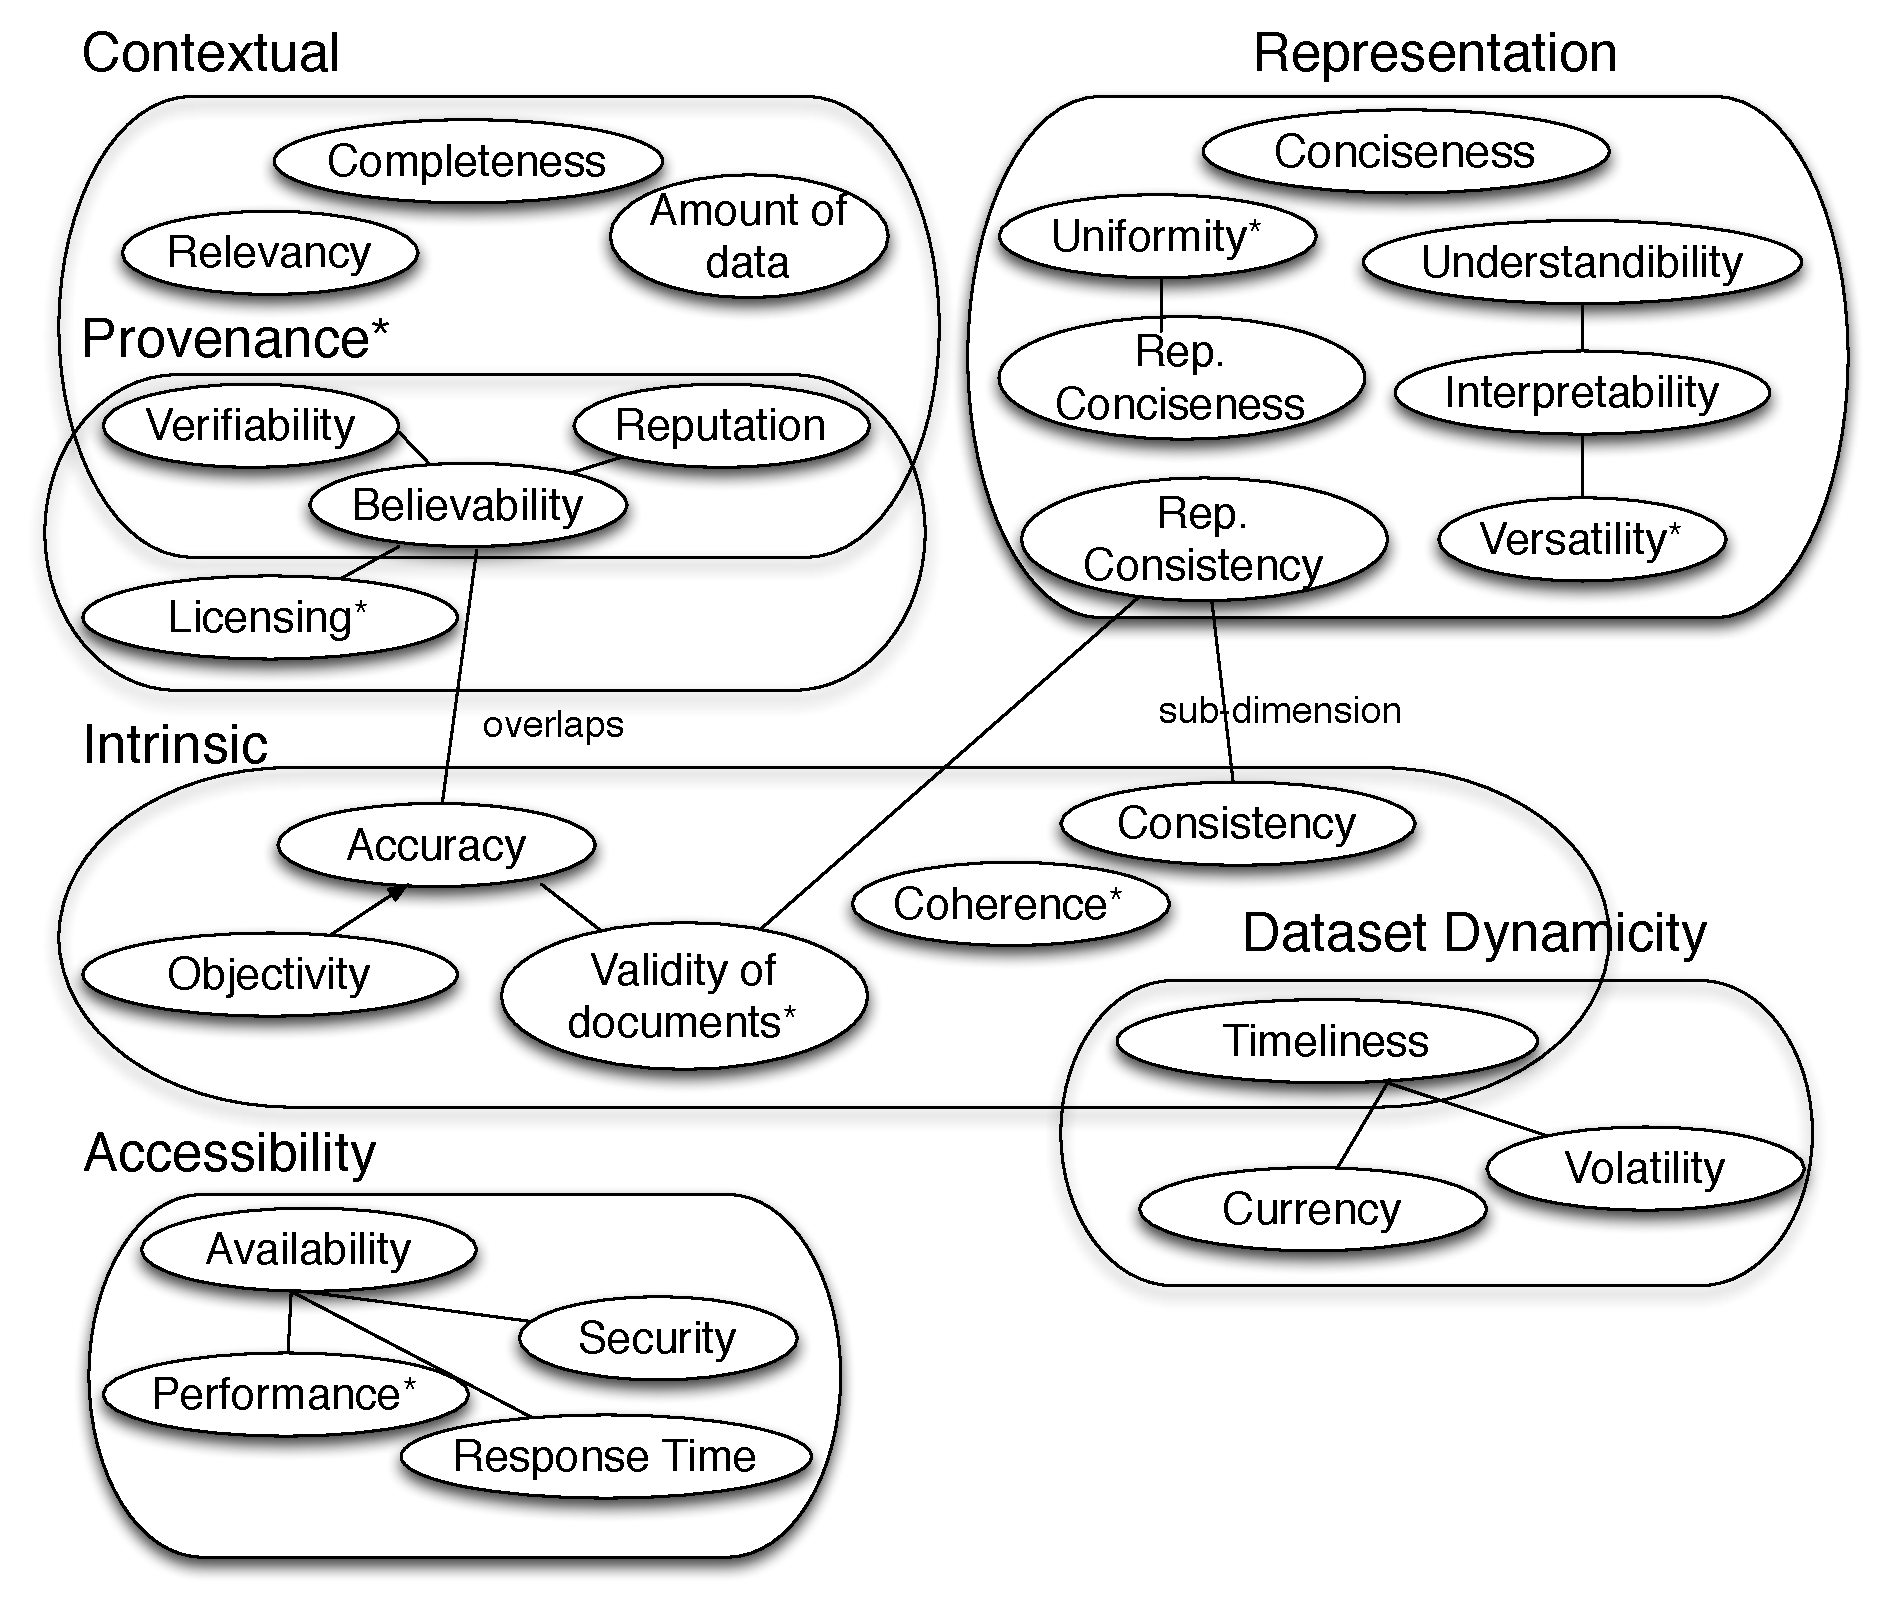
\includegraphics[width=5in]{DimensionsRelations.pdf}
\caption{Linked data quality dimensions and the relations between them.}
\label{fig:dimrel}
\end{figure*}
